\begin{figure*}[t]
  \centering
  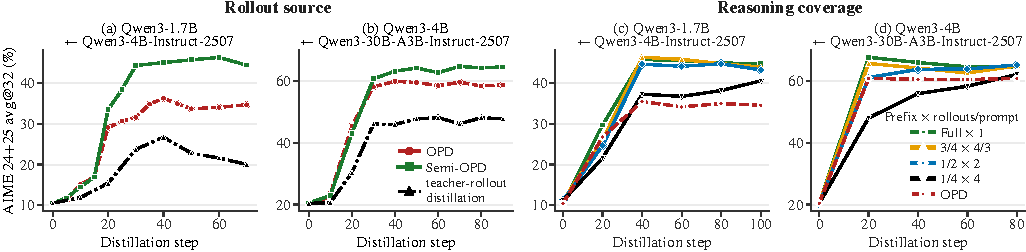
\includegraphics[width=\linewidth]{figures/fig_source_coverage.pdf}
  \vspace{-1em}
  \caption{
\textbf{rollout来源和推理覆盖对蒸馏都至关重要。}
\textbf{(a, b)} Semi-OPD在两组数据上均优于教师rollout蒸馏（以及OPD）。\textbf{(c, d)} 我们比较了在首个$1/4$、$1/2$、$3/4$或所有rollout阶段上训练的Semi-OPD，同时通过缩放每条提示的rollout数量来保持训练token总数不变。在所有阶段进行蒸馏的效果最佳。
}
  \label{fig:source_coverage}
  \label{fig:reasoning_coverage}
  \vspace{-0.5em}
\end{figure*}


\begin{figure}[t]
  \centering
  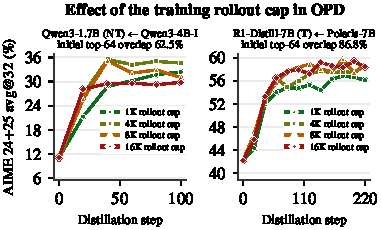
\includegraphics[width=\linewidth]{figures/fig_rollout_len.pdf}
  \vspace{-1.5em}
  \caption{
  更长的展开对重叠度低的一对（左）有负面影响，但对重叠度高的一对（右）没有影响。
  }
  \vspace{-1em}
  \label{fig:rollout_cap}
\end{figure}


\begin{figure*}[t]
  \centering
  \vspace{-0.5em}
  \begin{minipage}[t]{0.48\linewidth}
    \centering
    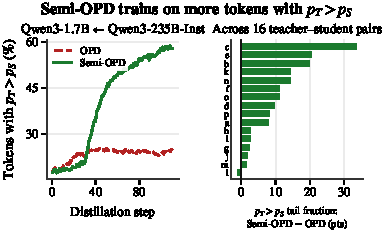
\includegraphics[width=\linewidth]{figures/fig_signal.pdf}
    \captionsetup{skip=4pt}
    \caption{\textbf{具有正奖励的token的百分比}，即在Semi-OPD和OPD下具有$p_T > p_S$的训练token的比例。}
    \label{fig:teacher_student_signal}
  \end{minipage}\hfill
  \begin{minipage}[t]{0.48\linewidth}
    \centering
    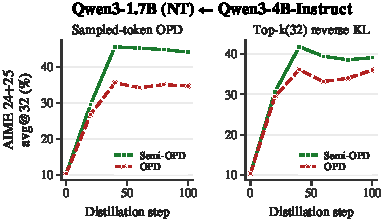
\includegraphics[width=\linewidth]{figures/fig_objective.pdf}
    \captionsetup{skip=4pt}
    \caption{\textbf{半监督OPD与OPD在两种蒸馏目标下的对比}，即，采样token和top-$k$ 逆KL目标。}
    \label{fig:distillation_objective}
  \end{minipage}
\end{figure*}


\begin{figure*}[t]
  \centering
  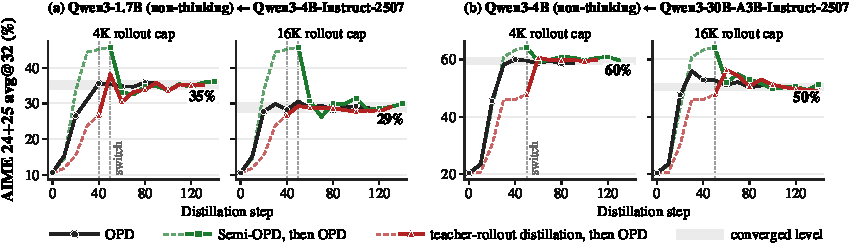
\includegraphics[width=\linewidth]{figures/fig_handoff.pdf}
    \vspace{-1.5em}
\caption{
\textbf{切换到OPD会趋向于一个由滚动预测决定的平衡状态，很大程度上与初始化无关。}
从初始学生模型、Semi-OPD检查点或教师滚动蒸馏检查点初始化时的OPD评估准确率轨迹。切换到OPD可能会降低或提升性能（见 \cref{fig:cache_switch_highoverlap}），其轨迹会趋近于在相同滚动上限下从头开始训练的OPD的性能水平。虚线表示切换到OPD之前的训练过程。
}
  \label{fig:handoff}
  \vspace{-1em}
\end{figure*}



\vspace{-0.5em}
\section{为什么OPD通常表现不如半透明OPD？}
\vspace{-0.5em}
\label{sec:why}

我们进一步探究了在重叠度较低的情况下，OPD性能不如Semi-OPD的原因。

\noindent \textbf{我们的假设。}
我们假设有效的蒸馏需要训练数据（即轨迹）满足两个特性：(1) 相对于学生模型的同策略性，以避免曝光偏差，以及 (2) 来自教师模型的高质量监督，这通常由相对于教师分布的同策略性决定，即轨迹与教师自身推理时分布的对齐程度。
同策略蒸馏（OPD）更注重前者，但在后者上表现不佳，尤其是在教师与学生之间重叠度较低的情况下；半同策略蒸馏（Semi-OPD）在一定程度上牺牲了学生模型的同策略性，以获得更有效的监督信号，如下文分析所示。

更具体地说，对于低重叠对，OPD 过程中的轨迹变得越来越长，并表现出各种伪影~\citep{luo2026demystifying, yang2026eos, fu2026revisiting}。这使得轨迹中较晚的 token 与教师的分布越来越偏离同策略，导致教师对这些 token 的监督变得无用甚至有害~\citep{xu2026pass,jiang2026trajectory}。  
截断轨迹并仅在前缀上进行训练可以缓解这一问题~\citep{zhang2026fast,ziheng2026less}，但代价是移除了对后期 token 的监督。如后续所示，在完整轨迹中覆盖所有推理阶段的监督信号对最终性能至关重要。  
相比之下，Semi-OPD 在初始学生生成的轨迹上进行训练，这些轨迹通常比同策略轨迹更短，从而在保持与教师分布的较好同策略性的同时，仍能覆盖包含所有推理阶段的完整轨迹。  
我们通过以下研究支持上述分析。


\noindent \textbf{学生同策略性的重要性：半同策略蒸馏与教师轨迹蒸馏对比。}
我们通过将初始学生轨迹缓存替换为教师生成的轨迹，同时保持其他所有情景不变，研究学生同策略性对半同策略蒸馏的影响。
如图~\ref{fig:source_coverage}(a, b)所示，半同策略蒸馏始终优于教师轨迹蒸馏。这表明半同策略蒸馏的优势并非仅仅来自于使用固定轨迹缓存。保留学生生成的轨迹以维持学生同策略性同样至关重要。




\noindent \textbf{在更长的回溯序列上进行训练可能会损害低重叠对的OPD表现。}  
如\cref{fig:rollout_cap}所示，我们调整了用于OPD训练的回溯序列长度（即回溯上限），观察到增加回溯上限会损害低重叠对的表现，而对高重叠对则有益。  
我们假设，对于低重叠对而言，在与教师策略异策略的长回溯序列上进行训练，可能倾向于强化表面化的推理模式，而未能充分改善潜在的推理过程，从而导致后续学生回溯序列的表现下降（回溯序列对比示例见附录~\ref{app:qualitative}）。


\noindent \textbf{覆盖所有推理阶段的监督信号至关重要。}  
如果长轨迹可能带来负面影响，一个简单的解决方案是截断它们，但这会损失后期推理阶段的监督信息。为隔离推理阶段覆盖的重要性，我们通过将缓存的半监督OPD迹（Semi-OPD traces）截断至其长度的前 $1/4$ 、$1/2$ 或 $3/4$ ，同时按比例调整每个提示的轨迹数量以保持总训练 token 预算不变，进行消融实验。如图~\ref{fig:reasoning_coverage}(c, d) 所示，仅保留前四分之一的监督会显著减慢收敛速度并降低最终准确率，而使用完整轨迹进行训练则达到最佳峰值准确率。因此，覆盖所有推理阶段以及保持与教师模型的同策略性均至关重要。




\noindent \textbf{Semi-OPD 使学生接触到更多教师偏好的 token。}  
Semi-OPD 通过较短的 rollout 长度实现完整轨迹覆盖，确切满足上述要求。为分析由此产生的蒸馏信号，我们测量训练过程中具有 $p_T > p_S$ 的 token 比例，即因教师赋予更高概率而获得正奖励的 token。  
如图~\ref{fig:teacher_student_signal} 所示，Semi-OPD 在整个训练过程中保持了比 OPD 更大比例的此类 token。这表明 Semi-OPD 使学生接触到更多教师偏好的 token，即相对于教师具有更高的同策略性，而 OPD 更常产生抑制学生自身采样 token 的信号。  
重要的是，如图~\ref{fig:distillation_objective} 所示，Semi-OPD 在 top-$k$ 反向 KL 下也优于 OPD，表明其优势并非仅针对采样 token 目标。


这些发现共同表明，半同策略动态（Semi-OPD）得益于保留对学生锚定的轨迹，这些轨迹能持续提供有效的教师监督，并广泛覆盖推理过程。在教师与学生模型差异较大的情况下，这些优势可超过完全同策略采样的好处。





































